% By J. Leon, Modified for improved clarity
\documentclass[tikz,border=10pt]{standalone}
\usepackage{tikz}
\usetikzlibrary{positioning, fit, arrows.meta, shapes}

% Define LSTM notation helper
\newcommand{\empt}[2]{$#1^{\langle #2 \rangle}$}

\begin{document}

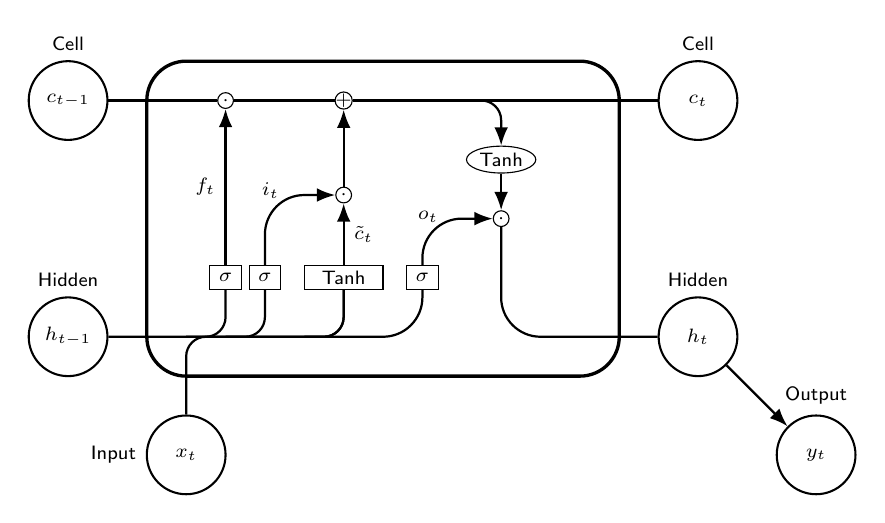
\begin{tikzpicture}[
    % GLOBAL CFG
    font=\sf \scriptsize,
    >=LaTeX,
    % Styles
    cell/.style={
        rectangle, 
        rounded corners=5mm, 
        draw,
        very thick,
    },
    operator/.style={
        circle,
        draw,
        inner sep=-0.5pt,
        minimum height =.2cm,
    },
    function/.style={
        ellipse,
        draw,
        inner sep=1pt
    },
    ct/.style={
        circle,
        draw,
        line width = .75pt,
        minimum width=1cm,
        inner sep=1pt,
    },
    gt/.style={
        rectangle,
        draw,
        minimum width=4mm,
        minimum height=3mm,
        inner sep=1pt
    },
    mylabel/.style={
        font=\scriptsize\sffamily
    },
    ArrowC1/.style={
        rounded corners=.25cm,
        thick,
    },
    ArrowC2/.style={
        rounded corners=.5cm,
        thick,
    },
]

% Start drawing the thing...    
    % Draw the cell: 
    \node [cell, minimum height =4cm, minimum width=6cm] at (0,0){} ;

    % Draw inputs named ibox#
    \node [gt] (ibox1) at (-2,-0.75) {$\sigma$};
    \node [gt] (ibox2) at (-1.5,-0.75) {$\sigma$};
    \node [gt, minimum width=1cm] (ibox3) at (-0.5,-0.75) {Tanh};
    \node [gt] (ibox4) at (0.5,-0.75) {$\sigma$};

   % Draw operators named mux#, add# and func#
    \node [operator] (mux1) at (-2,1.5) {$\cdot$};
    \node [operator] (add1) at (-0.5,1.5) {+};
    \node [operator] (mux2) at (-0.5,0.3) {$\cdot$};
    \node [operator] (mux3) at (1.5,0) {$\cdot$};
    \node [function] (func1) at (1.5,0.75) {Tanh};

    % Draw External inputs named as basis c,h,x
    \node[ct, label={[mylabel]Cell}] (c) at (-4,1.5) {$c_{t-1}$};
    \node[ct, label={[mylabel]Hidden}] (h) at (-4,-1.5) {$h_{t-1}$};
    \node[ct, label={[mylabel]left:Input}] (x) at (-2.5,-3) {$x_t$};

    % Draw External outputs named as basis c2,h2,x2
    \node[ct, label={[mylabel]Cell}] (c2) at (4,1.5) {$c_t$};
    \node[ct, label={[mylabel]Hidden}] (h2) at (4,-1.5) {$h_t$};
    \node[ct, label={[mylabel]Output}] (y) at (5.5,-3) {$y_t$};  % Added y_t output

% Start connecting all.
    % Intersections and displacements are used. 
    % Drawing arrows    
    \draw [ArrowC1] (c) -- (mux1) -- (add1) -- (c2);

    % Inputs
    \draw [ArrowC2] (h) -| (ibox4);
    \draw [ArrowC1] (h -| ibox1)++(-0.5,0) -| (ibox1); 
    \draw [ArrowC1] (h -| ibox2)++(-0.5,0) -| (ibox2);
    \draw [ArrowC1] (h -| ibox3)++(-0.5,0) -| (ibox3);
    \draw [ArrowC1] (x) -- (x |- h)-| (ibox3);

    % Internal
    \draw [->, ArrowC2] (ibox1) -- (mux1) node[midway, left] {$f_t$};
    \draw [->, ArrowC2] (ibox2) |- (mux2) node[midway, above, yshift=-5pt, xshift=2pt] {$i_t$};
    \draw [->, ArrowC2] (ibox3) -- (mux2) node[midway, right] {$\tilde{c}_t$};
    \draw [->, ArrowC2] (ibox4) |- (mux3) node[midway, above, yshift=-5pt, xshift=2pt] {$o_t$};
    \draw [->, ArrowC2] (mux2) -- (add1);
    \draw [->, ArrowC1] (add1 -| func1)++(-0.5,0) -| (func1);
    \draw [->, ArrowC2] (func1) -- (mux3);

    % Outputs
    \draw [-, ArrowC2] (mux3) |- (h2);
    %\draw [ArrowC2,blue] (c2 -| h2) ++(0,-0.8) coordinate (i1);
    %\draw [-, ArrowC2, red] (h2.north) |- (i1);
    
    % Arrow from h_t to y_t
    \draw [->, thick] (h2) -- (y);

\end{tikzpicture}

\end{document}
